\subsection{Insegnante}

\subsubsection{Panoramica insegnante}
\begin{comment}
\begin{figure}[H]
\centering
\includegraphics[width=17cm, height=20cm]{img/} 
\caption{Panoramica insegnante}
\end{figure}
\end{comment}


\subsubsection{UC 2.1 - Visualizzazione della dashboard}
\begin{itemize}
	\item[•] \textbf{Attori}: Insegnante;
	\item[•] \textbf{Descrizione}: l’insegnante accede alla propria dashboard;
	\item[•] \textbf{Precondizione}: l'insegnante si è autenticato;
	\item[•] \textbf{Postcondizione}: l'insegnante visualizza tutti i componenti della sua dashboard;
	\item[•] \textbf{Flusso degli eventi}: l’insegnante ha effettuato il login e viene reindirizzato alla propria dashboard.
\end{itemize}

\subsubsection{UC 2.2 - Inserimento di un nuovo esercizio}

\begin{comment}
\begin{figure}[H]
	\centering
	\includegraphics[width=17cm]{img/} 
	\caption{Caso d'uso UC 2.2;}
\end{figure}
\end{comment}

\begin{itemize}
	\item[•] \textbf{Attori}: Insegnante;
	\item[•] \textbf{Descrizione}: l'insegnante aggiunge un nuovo esercizio. 
	\item[•] \textbf{Precondizione}: l'insegnante si è autenticato e visualizza la propria dashboard;
	\item[•] \textbf{Postcondizione}: l'insegnante ha inserito un esercizio;
	\item[•] \textbf{Flusso degli eventi}:
	\begin{enumerate}
		\item UC 2.2.1 - Selezione lingua esercizio;
		\item UC 2.2.2 - Inserimento testo esercizio;
		\item UC 2.2.3 - Visualizzazione analisi automatica;
		\item UC 2.2.4 - Modifica tag automatico;
		\item UC 2.2.6 - Modifica visibilità esercizio;
		\item UC 2.2.7 - Assegna esercizio;
		\item UC 2.2.9 - Conferma aggiunta esercizio.
	\end{enumerate}
	\item[•] \textbf{Estensioni}:	
	\begin{enumerate}
		\item UC 2.2.2.1 - Visualizzazione errori sintassi testo;
		\item UC 2.2.8 - Interruzione inserimento esercizio.
	\end{enumerate}
	\item[•] \textbf{Flusso degli eventi alternativo}:
	\begin{enumerate}
		\item UC 2.2.5 - Aggiunta tag alternativo.
	\end{enumerate}
\end{itemize}
 

\subsubsection{UC 2.2.1 - Selezione lingua esercizio}
\begin{itemize}
	\item[•] \textbf{Attori}: Insegnante;
	\item[•] \textbf{Descrizione}: l'insegnante sceglie la lingua dell'esercizio che vuole scrivere;
	\item[•] \textbf{Precondizione}: l'insegnante sta inserendo un esercizio;
	\item[•] \textbf{Postcondizione}: l'insegnante ha scelto la lingua dell'esercizio;
	\item[•] \textbf{Flusso degli eventi}: l'insegnante durante l'inserimento di un esercizio sceglie la lingua dell'esercizio.
\end{itemize}

\subsubsection{UC 2.2.2 - Inserimento testo esercizio}
\begin{itemize}
	\item[•] \textbf{Attori}: Insegnante;
	\item[•] \textbf{Descrizione}: l'insegnante scrive il testo dell'esercizio;
	\item[•] \textbf{Precondizione}: l'insegnante sta inserendo un esercizio;
	\item[•] \textbf{Postcondizione}: l'insegnante ha inserito il testo dell'esercizio;
	\item[•] \textbf{Flusso degli eventi}: l'insegnante durante l'inserimento di un esercizio scrive il testo dell'esercizio.
\end{itemize}

\subsubsection{UC 2.2.2.1 - Visualizzazione errori sintassi testo}
\begin{itemize}
	\item[•] \textbf{Attori}: Insegnante;
	\item[•] \textbf{Descrizione}: l'insegnante visualizza gli errori relativi alla sintassi e la forma del testo che ha inserito;
	\item[•] \textbf{Precondizione}: l'insegnante sta inserendo un esercizio;
	\item[•] \textbf{Postcondizione}: l'insegnante visualizza gli errori relativi al testo inserito;
	\item[•] \textbf{Flusso degli eventi}: l'insegnante durante l'inserimento del testo, commette un errore di sintassi.
\end{itemize}

\subsubsection{UC 2.2.3 - Visualizzazione analisi automatica} 
\begin{itemize}
	\item[•] \textbf{Attori}: Insegnante;
	\item[•] \textbf{Descrizione}: l'insegnante visualizza l'analisi automatica;
	\item[•] \textbf{Precondizione}: l'insegnante sta inserendo un esercizio;
	\item[•] \textbf{Postcondizione}: l'insegnante visualizza l'analisi automatica generata per il testo inserito;
	\item[•] \textbf{Flusso degli eventi}: l'insegnante durante l'inserimento di un esercizio, riceve una correzione automatica e ne visualizza il contenuto.
\end{itemize}


\subsubsection{UC 2.2.4 - Modifica tag automatico}
\begin{itemize}
	\item[•] \textbf{Attori}: Insegnante;
	\item[•] \textbf{Descrizione}: l'insegnante modifica uno o più tag per parola;
	\item[•] \textbf{Precondizione}: l'insegnante visualizza la soluzione dell'esercizio proposta dal sistema automatico di correzione;
	\item[•] \textbf{Postcondizione}: l'insegnante ha modificato uno o più tag generati automaticamente;
\item[•] \textbf{Flusso degli eventi}:
\begin{enumerate}
		\item Selezione tag da modificare;
		\item Selezione tag corretto.
\end{enumerate}
\end{itemize}

\subsubsection{UC 2.2.5 - Aggiunta tag alternativo}
\begin{itemize}
	\item[•] \textbf{Attori}: Insegnante;
	\item[•] \textbf{Descrizione}: l'insegnante aggiunge uno o più tag alternativi per parola;
	\item[•] \textbf{Precondizione}: l'insegnante visualizza la soluzione dell'esercizio proposta dal sistema automatico di correzione;
	\item[•] \textbf{Postcondizione}: l'insegnante ha aggiunto uno o più tag alternativi (oltre a quelli principali) per una o più parole;
\item[•] \textbf{Flusso degli eventi}:
\begin{enumerate}
		\item Selezione tag per aggiunta alternativa;
		\item Selezione tag alternativo.
\end{enumerate}
\end{itemize}


\subsubsection{UC 2.2.6 - Modifica visibilità esercizio}
\begin{itemize}
	\item[•] \textbf{Attori}: Insegnante;
	\item[•] \textbf{Descrizione}: l'insegnante imposta la visibilità dell'esercizio, ovvero quali allievi o classi possono visualizzarlo e sceglierlo;
	\item[•] \textbf{Precondizione}: l'insegnante sta inserendo un esercizio;
	\item[•] \textbf{Postcondizione}: l'insegnante ha modificato la visibilità dell'esercizio;
	\item[•] \textbf{Flusso degli eventi}: l'insegnante sceglie (tra le visibilità proposte) che visibilità dare all'esercizio.
\end{itemize}


\subsubsection{UC 2.2.7 - Assegna esercizio} 
\begin{itemize}
	\item[•] \textbf{Attori}: Insegnante;
	\item[•] \textbf{Descrizione}: l'insegnante assegna un esercizio ad un alunno o una classe;
	\item[•] \textbf{Precondizione}: l'insegnante sta inserendo un esercizio;;
	\item[•] \textbf{Postcondizione}: l'insegnante ha assegnato l'esercizio ad un alunno o una classe (gruppo di alunni);
	\item[•] \textbf{Flusso degli eventi}: l'insegnante durante l'inserimento di un esercizio decide a chi assegnarlo, se un alunno specifico o una classe di alunni.
\end{itemize}

\subsubsection{UC 2.2.8 - Interruzione inserimento esercizio}
\begin{itemize}
	\item[•] \textbf{Attori}: Insegnante;
	\item[•] \textbf{Descrizione}: l'insegnante interrompe l'inserimento di un esercizio;
	\item[•] \textbf{Precondizione}: l'insegnante sta inserendo un esercizio;;
	\item[•] \textbf{Postcondizione}: l'esercizio non è stato inserito;
	\item[•] \textbf{Flusso degli eventi}: l'insegnante durante l'inserimento di un esercizio decide di annullarlo (o viene annullato), pertanto l'esercizio non viene aggiunto al sistema.
\end{itemize}

\subsubsection{UC 2.2.9 - Conferma aggiunta esercizio}
\begin{itemize}
	\item[•] \textbf{Attori}: Insegnante;
	\item[•] \textbf{Descrizione}: l'insegnante conferma l'inserimento dell'esercizio;
	\item[•] \textbf{Precondizione}: l'insegnante sta inserendo un esercizio;
	\item[•] \textbf{Postcondizione}: l'insegnante aggiunge un esercizio al sistema;
	\item[•] \textbf{Flusso degli eventi}:l'insegnante ha completato e selezionato tutti i campi presenti ed ha confermato l'aggiunta dell'esercizio.
\end{itemize}


\subsubsection{UC 2.3 - Visualizzazione storico frasi inserite}
\begin{itemize}
	\item[•] \textbf{Attori}: Insegnante	   
	\item[•] \textbf{Descrizione}: l'insegnante visualizza lo storico delle frasi inserite sotto forma tabellare; 
	\item[•] \textbf{Precondizione}: l'insegnante sta visualizzando la propria dashboard;
	\item[•] \textbf{Postcondizione}: l'insegnante naviga all'interno della lista di frasi che ha inserito;
	\item[•] \textbf{Flusso degli eventi}: l'insegnante seleziona l'apposito campo per la visualizzazione dello storico frasi inserite.
\end{itemize}


\subsubsection{UC 2.3.1 - Visualizzazione dettaglio esercizio}
\begin{itemize}
	\item[•] \textbf{Attori}: Insegnante;
	\item[•] \textbf{Descrizione}: l'insegnante seleziona dalla lista degli esercizi assegnati un esercizio e ne visualizza i dettagli: nome e cognome dell'allievo che ha svolto l'esercizio;
	\item[•] \textbf{Precondizione}: l'insegnante visualizza la lista di frasi che ha inserito;
	\item[•] \textbf{Postcondizione}: l'insegnante visualizza i dettagli di un esercizio inserito;
	\item[•] \textbf{Flusso degli eventi}: l'insegnante naviga all'interno della lista di frasi che ha inserito e seleziona un esercizio specifico.
\end{itemize}


\subsubsection{UC 2.4 - Visualizzazione esercizi svolti dagli allievi}
\begin{itemize}
	\item[•] \textbf{Attori}: Insegnante;
	\item[•] \textbf{Descrizione}:  l'insegnante visualizza l'elenco degli esercizi svolti dagli allievi;
	\item[•] \textbf{Precondizione}: l'insegnante visualizza la propria dashboard;
	\item[•] \textbf{Postcondizione}: l'insegnante naviga all'interno della lista di esercizi svolti;
	\item[•] \textbf{Flusso degli eventi}: l'insegnante seleziona l'apposito campo per la visualizzazione degli esercizi svolti dai propri allievi.
\end{itemize}

\subsubsection{UC 2.5 - Visualizzazione dei propri allievi}
\begin{itemize}
	\item[•] \textbf{Attori}: Insegnante;
	\item[•] \textbf{Descrizione}: l'insegnante visualizza la lista dei suoi allievi: nome, cognome, data di nascita, classe di appartenenza e insegnante preferito;
	\item[•] \textbf{Precondizione}: l'insegnante visualizza la propria dashboard;
	\item[•] \textbf{Postcondizione}: l'insegnante visualizza la lista dei propri allievi;
	\item[•] \textbf{Flusso degli eventi}:  l'insegnante seleziona l'apposito campo per la visualizzazione della lista dei propri allievi.
\end{itemize}


\subsubsection{UC 2.6 - Modifica esercizio}


\begin{comment}
\begin{figure}[H]
\centering
\includegraphics[width=17cm]{img/} 
\caption{Caso d'uso UC 2.6}
\end{figure}
\end{comment}

\begin{itemize}
	\item[•] \textbf{Attori}: Insegnante;
	\item[•] \textbf{Descrizione}: l'insegnante può modificare il testo, i tag automatici e la visibilità, inoltre può eliminare un tag alternativo e riassegnare un esercizio precedentemente inserito;
	\item[•] \textbf{Precondizione}:  l'insegnante visualizza la propria dashboard;
	\item[•] \textbf{Postcondizione}: l'insegnante ha modificato l'esercizio;
	\item[•] \textbf{Flusso degli eventi}:
	\begin{enumerate}
		\item Selezione procedura modifica esercizio;
		\item UC 2.6.1 - Modifica testo esercizio;
		\item UC 2.6.2 - Modifica tag automatico;
		\item UC 2.6.3 - Modifica visibilità;
		\item UC 2.6.4 - Riassegnazione esercizio;
		\item UC 2.6.5 - Eliminazione tag alternativo;
		\item UC 2.6.7 - Salvataggio modifiche.
	\end{enumerate}
	\item[•] \textbf{Estensioni}:	
	\begin{enumerate}
		\item UC 2.6.6 - Annullamento modifiche.
	\end{enumerate}
\end{itemize}


\subsubsection{UC 2.6.1 - Modifica testo esercizio}
\begin{itemize}
	\item[•] \textbf{Attori}: Insegnante;
	\item[•] \textbf{Descrizione}: l'insegnante modifica il testo di un esercizio;
	\item[•] \textbf{Precondizione}: l'insegnante sta modificando un esercizio;
	\item[•] \textbf{Postcondizione}: l'insegnante ha modificato il testo dell'esercizio;
	\item[•] \textbf{Flusso degli eventi}: l'insegnante modifica il testo di un esercizio precedentemente inserito.
\end{itemize}


\subsubsection{UC 2.6.2 - Modifica tag automatico}
\begin{itemize}
	\item[•] \textbf{Attori}: Insegnante;
	\item[•] \textbf{Descrizione}: l'insegnante modifica uno o più tag per parola;
	\item[•] \textbf{Precondizione}: l'insegnante sta modificando un esercizio;
	\item[•] \textbf{Postcondizione}: l'insegnante ha modificato uno o più tag precedentemente inseriti;
\item[•] \textbf{Flusso degli eventi}:
\begin{enumerate}
		\item Selezione tag da modificare;
		\item Selezione tag corretto.
\end{enumerate}
\end{itemize}


\subsubsection{UC 2.6.3 - Modifica visibilità} 
\begin{itemize}
	\item[•] \textbf{Attori}: Insegnante;
	\item[•] \textbf{Descrizione}: l'insegnante modifica la visibilità di un esercizio;
	\item[•] \textbf{Precondizione}: l'insegnante sta modificando un esercizio;
	\item[•] \textbf{Postcondizione}: l'insegnante ha modificato la visibilità dell'esercizio;
	\item[•] \textbf{Flusso degli eventi}: l'insegnante modifica la visibilità dell'esercizio.
\end{itemize}


\subsubsection{UC 2.6.4 - Riassegnazione esercizio}
\begin{itemize}
	\item[•] \textbf{Attori}: Insegnante;
	\item[•] \textbf{Descrizione}: l'insegnante riassegna un esercizio;
	\item[•] \textbf{Precondizione}:  l'insegnante sta modificando un esercizio;
	\item[•] \textbf{Postcondizione}: l'insegnante ha riassegnato l'esercizio;
	\item[•] \textbf{Flusso degli eventi}: l'insegnante riassegna ad un diverso alunno o ad una diversa classe l'esercizio precedentemente inserito.
\end{itemize}


\subsubsection{UC 2.6.5 - Eliminazione tag alternativo}
\begin{itemize}
	\item[•] \textbf{Attori}: Insegnante;
	\item[•] \textbf{Descrizione}: l'insegnante elimina uno o più tag alternativi;
	\item[•] \textbf{Precondizione}: l'insegnante sta modificando un esercizio;
	\item[•] \textbf{Postcondizione}: l'insegnante ha eliminato uno o più tag alternativi di un esercizio.
	\item[•] \textbf{Flusso degli eventi}:
\begin{enumerate}
		\item Selezione tag da eliminare;
		\item elimina tag.
\end{enumerate}
\end{itemize}

\subsubsection{UC 2.6.6 - Annullamento modifiche}
\begin{itemize}
	\item[•] \textbf{Attori}: Insegnante;
	\item[•] \textbf{Descrizione}: l'insegnante annulla le modifiche inserite all'interno di un esercizio; 
	\item[•] \textbf{Precondizione}: l'insegnante sta modificando un esercizio;
	\item[•] \textbf{Postcondizione}: l'esercizio non è modificato.
	\item[•] \textbf{Flusso degli eventi}:l'insegnante interrompe la procedura di modifica, le modifiche non vengono apportate al sistema.
\end{itemize}

\subsubsection{UC 2.6.7 - Salvataggio modifiche.} 
\begin{itemize}
	\item[•] \textbf{Attori}: Insegnante;
	\item[•] \textbf{Descrizione}: l'insegnante salve le proprie modifiche;
	\item[•] \textbf{Precondizione}: l'insegnante ha modificato uno o più campi dell'esercizio;
	\item[•] \textbf{Postcondizione}: l'insegnante ha salvato le modifiche;
	\item[•] \textbf{Flusso degli eventi}: l'insegnante dopo aver apportato le opportune modifiche salva i cambiamenti che vengono aggiornati nel sistema.
\end{itemize}


\subsubsection{UC 2.7 - Eliminazione esercizio}
\begin{itemize}
	\item[•] \textbf{Attori}: Insegnante;
	\item[•] \textbf{Descrizione}: l'insegnante ha la possibilità di eliminare un esercizio precedentemente inserito;
	\item[•] \textbf{Precondizione}: l'insegnante visualizza lo storico delle frasi inserite;
	\item[•] \textbf{Postcondizione}: l'insegnante ha eliminato l'esercizio precedentemente inserito;
	\item[•] \textbf{Flusso degli eventi}:l'insegnante seleziona un esercizio specifico dalla lista dello storico frasi e seleziona l'apposito campo per l'eliminazione.
\end{itemize}


\subsubsection{UC 2.8 - Modifica dati utente}
\begin{itemize}
	\item[•] \textbf{Attori}: Insegnante;
	\item[•] \textbf{Descrizione}: l'insegnante modifica i propri dati personali, cioè tutti i dati inseriti in fase di registrazione;
	\item[•] \textbf{Precondizione}: l'insegnante visualizza la propria dashboard;
	\item[•] \textbf{Postcondizione}: l'insegnante ha modificato uno o più dati personali;
	\item[•] \textbf{Flusso degli eventi}:
	\begin{enumerate}
		\item Selezione procedura modifica dati personali;
		\item UC 2.8.1 - Modifica email ;
		\item UC 2.8.2 - Modifica nome;
		\item UC 2.8.3 - Modifica cognome;
		\item UC 2.8.4 - Modifica password
		\item UC 2.8.5 - Modifica data di nascita;
		\item UC 2.8.6 - Modifica lingua interfaccia applicativo;
		\item UC 2.8.7 - Conferma modifica dati.
	\end{enumerate}
\end{itemize}

\subsubsection{UC 2.8.1 - Modifica email}
\begin{itemize}
	\item[•]\textbf{Attori}: Insegnante;
	\item[•]\textbf{Descrizione}: l'insegnante modifica la propria email;
	\item[•]\textbf{Precondizione}: l'insegnante sta modificando i propri dati personali;
	\item[•]\textbf{Postcondizione}: l'insegnante ha modificato la propria email; 
	\item[•]\textbf{Flusso degli eventi}: 
	\begin{enumerate}
		\item Selezione campo email;
		\item Modifica la stringa che rappresenta la propria email.
	\end{enumerate}
\end{itemize}

\subsubsection{UC 2.8.2 - Modifica nome}
\begin{itemize}
	\item[•]\textbf{Attori}: Insegnante;
	\item[•]\textbf{Descrizione}: l'insegnante modifica il proprio nome;
	\item[•]\textbf{Precondizione}: l'insegnante sta modificando i propri dati personali;
	\item[•]\textbf{Postcondizione}: l'insegnante ha modificato il proprio nome; 
	\item[•]\textbf{Flusso degli eventi}: 
	\begin{enumerate}
		\item Selezione campo nome;
		\item Modifica la stringa che rappresenta il proprio nome.
	\end{enumerate}
\end{itemize}

\subsubsection{UC 2.8.3 - Modifica cognome}
\begin{itemize}
	\item[•]\textbf{Attori}: Insegnante;
	\item[•]\textbf{Descrizione}: l'insegnante modifica il proprio cognome;
	\item[•]\textbf{Precondizione}: l'insegnante sta modificando i propri dati personali;
	\item[•]\textbf{Postcondizione}: l'insegnante ha modificato il proprio cognome; 
	\item[•]\textbf{Flusso degli eventi}: 
	\begin{enumerate}
		\item Selezione campo cognome;
		\item Modifica la stringa che rappresenta il proprio cognome.
	\end{enumerate}
\end{itemize}


\subsubsection{UC 2.8.4 - Modifica password}
\begin{itemize}
	\item[•]\textbf{Attori}: Insegnante;
	\item[•]\textbf{Descrizione}: l'insegnante modifica la propria password;
	\item[•]\textbf{Precondizione}: l'insegnante sta modificando i propri dati personali;
	\item[•]\textbf{Postcondizione}: l'insegnante ha modificato la propria password; 
	\item[•]\textbf{Flusso degli eventi}: 
	\begin{enumerate}
		\item UC 2.8.4.1 Inserimento nuova Password;
		\item UC 2.8.4.2 Inserimento conferma nuova password.
	\end{enumerate}
\end{itemize}

\subsubsection{UC 2.8.4.1 Inserimento nuova Password}
\begin{itemize}
	\item[•] \textbf{Attori}: Insegnante;
	\item[•] \textbf{Descrizione}: l'insegnante
	\item[•] \textbf{Precondizione}: l'insegnante
	\item[•] \textbf{Postcondizione}: l'insegnante
	\item[•] \textbf{Flusso degli eventi}: 
\end{itemize}

\subsubsection{UC 2.8.4.2 Inserimento conferma nuova password}
\begin{itemize}
	\item[•] \textbf{Attori}: Insegnante;
	\item[•] \textbf{Descrizione}: l'insegnante
	\item[•] \textbf{Precondizione}: l'insegnante
	\item[•] \textbf{Postcondizione}: l'insegnante
	\item[•] \textbf{Flusso degli eventi}: 
\end{itemize}

	
	
\subsubsection{UC 2.8.5 - Modifica data di nascita}
\begin{itemize}
	\item[•]\textbf{Attori}: Insegnante;
	\item[•]\textbf{Descrizione}: l'insegnante modifica la propria data di nascita;
	\item[•]\textbf{Precondizione}: l'insegnante sta modificando i propri dati personali;
	\item[•]\textbf{Postcondizione}: l'insegnante ha modificato la propria data di nascita; 
	\item[•]\textbf{Flusso degli eventi}: 
	\begin{enumerate}
		\item Selezione campo data di nascita;
		\item Modifica la stringa che rappresenta la data di nascita, inserendo il valore corretto.
	\end{enumerate}
\end{itemize}

\subsubsection{UC 2.8.6 Modifica lingua interfaccia applicativo}
\begin{itemize}
	\item[•]\textbf{Attori}: Insegnante;
	\item[•]\textbf{Descrizione}: l'insegnante modifica la lingua dell'applicativo;
	\item[•]\textbf{Precondizione}: l'insegnante sta modificando i propri dati personali;
	\item[•]\textbf{Postcondizione}: l'insegnante ha modificato la lingua dell'applicativo; 
	\item[•]\textbf{Flusso degli eventi}: 
	\begin{enumerate}
		\item Selezione campo dati lingua applicativo;
		\item Selezione da un elenco predefinito la lingua dell'applicativo desiderata.
	\end{enumerate}
\end{itemize}

\subsubsection{UC 2.8.7 - Conferma modifica dati}
\begin{itemize}
	\item[•] \textbf{Attori}: Insegnante;
	\item[•] \textbf{Descrizione}: l'insegnante
	\item[•] \textbf{Precondizione}: l'insegnante
	\item[•] \textbf{Postcondizione}: l'insegnante
	\item[•] \textbf{Flusso degli eventi}: 
\end{itemize}
















\subsubsection{UC 2.9 - Visualizzazione elenco classi}
\begin{itemize}
	\item[•] \textbf{Attori}: Insegnante;
	\item[•] \textbf{Descrizione}: l'insegnante visualizza l'elenco delle classi;
	\item[•] \textbf{Precondizione}: l'insegnante si è autenticato e visualizza la propria dashboard;
	\item[•] \textbf{Postcondizione}: l'insegnante naviga all'interno della lista delle classi;
	\item[•] \textbf{Flusso degli eventi}: l'insegnante seleziona l'apposito campo per la visualizzazione delle proprie classi.
\end{itemize}

\subsubsection{UC 2.9.1 - Crea nuova classe}
\begin{figure}[H]
	\centering
	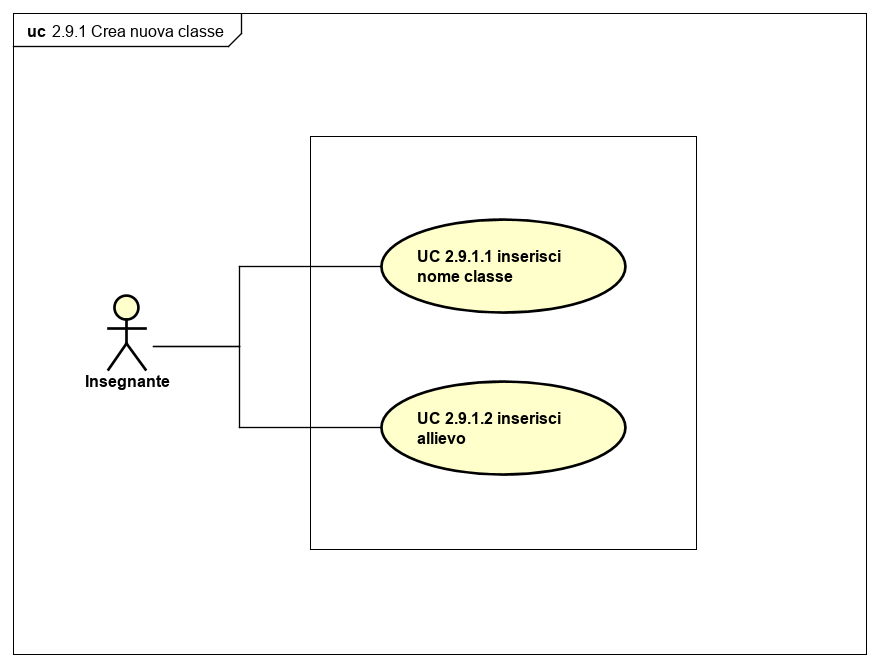
\includegraphics[width=17cm]{img/Crea_nuova_classe.png} 
	\caption{Caso d'uso UC 2.9.1;}
\end{figure}

\begin{itemize}
	\item[•] \textbf{Attori}: Insegnante;
	\item[•] \textbf{Descrizione}: l'insegnante crea una nuova classe di alunni;
	\item[•] \textbf{Precondizione}: l'insegnante visualizza l'elenco delle classi;
	\item[•] \textbf{Postcondizione}: l'insegnante ha creato una nuova classe di alunni;
	\item[•] \textbf{Flusso degli eventi}:
	\begin{enumerate}
		\item UC 2.9.1.1 inserisci nome classe;
		\item UC 2.9.1.2 inserisci allievo.
	\end{enumerate}
	\item[•] \textbf{Flusso degli eventi alternativo}:
	\begin{enumerate}
		\item UC 2.9.1.3 rimuovi allievo.
	\end{enumerate}
\end{itemize}

\begin{figure}[H]
	\centering
	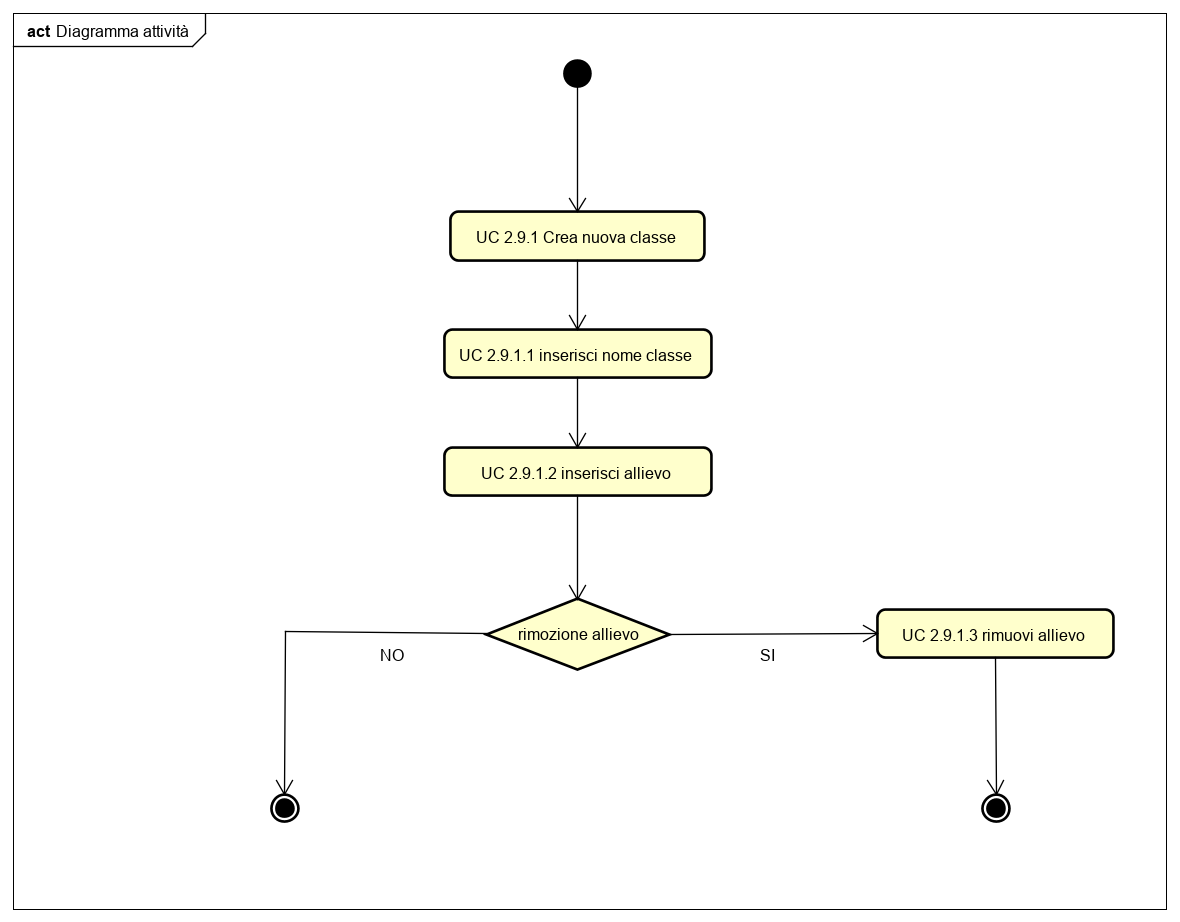
\includegraphics[width=17cm]{img/Diagramma_attivita_crea_classe.png} 
	\caption{Diagramma attività UC 2.9.1;}
\end{figure}


\subsubsection{UC 2.9.1.1 inserisci nome classe}
\begin{itemize}
	\item[•] \textbf{Attori}: Insegnante;
	\item[•] \textbf{Descrizione}: l'insegnante inserisce un nome della classe;
	\item[•] \textbf{Precondizione}: l'insegnante sta creando una classe;
	\item[•] \textbf{Postcondizione}: l'insegnante ha inserito il nome della classe che vuole creare;
	\item[•] \textbf{Flusso degli eventi}: l'insegnante durante la creazione di una classe inserisce il nome della classe.
\end{itemize}

\subsubsection{UC 2.9.1.2 inserisci allievo}
\begin{itemize}
	\item[•] \textbf{Attori}: Insegnante;
	\item[•] \textbf{Descrizione}: l'insegnante inserisce un allievo alla classe;
	\item[•] \textbf{Precondizione}: l'insegnante sta creando una classe;
	\item[•] \textbf{Postcondizione}: l'insegnante ha inserito un allievo alla classe;
	\item[•] \textbf{Flusso degli eventi}: l'insegnante durante la creazione di una classe inserisce un nuovo allievo al suo interno.
\end{itemize}

\subsubsection{UC 2.9.1.3 rimuovi allievo}
\begin{itemize}
	\item[•] \textbf{Attori}: Insegnante;
	\item[•] \textbf{Descrizione}: l'insegnante rimuove un allievo dalla classe;
	\item[•] \textbf{Precondizione}: l'insegnante ha aggiunto almeno un allievo alla classe;
	\item[•] \textbf{Postcondizione}: l'insegnante ha rimosso l'allievo dalla classe;
	\item[•] \textbf{Flusso degli eventi}: l'insegnante durante la creazione di una classe inserisce per errore un nuovo allievo al suo interno per poi rimuoverlo.
\end{itemize}


\subsubsection{UC 2.9.2 modifica classe}
\begin{itemize}
	\item[•] \textbf{Attori}: Insegnante;
	\item[•] \textbf{Descrizione}: l'insegnante modifica una classe ;
	\item[•] \textbf{Precondizione}: l'insegnante visualizza l'elenco delle classi;
	\item[•] \textbf{Postcondizione}: l'insegnante ha modificato uno o più campi della classe ;
	\item[•] \textbf{Flusso degli eventi}:
	\begin{enumerate}
		\item UC 2.9.2.1 modifica nome classe;
		\item UC 2.9.2.2 inserisci allievo.
	\end{enumerate}
	\item[•] \textbf{Flusso degli eventi alternativo}:
	\begin{enumerate}
		\item UC 2.9.2.3 rimuovi allievo.
	\end{enumerate}
\end{itemize}

\subsubsection{UC 2.9.2.1 modifica nome classe}
\begin{itemize}
	\item[•] \textbf{Attori}: Insegnante;
	\item[•] \textbf{Descrizione}: l'insegnante modifica il nome di una classe;
	\item[•] \textbf{Precondizione}: l'insegnante sta modificando una classe;
	\item[•] \textbf{Postcondizione}: l'insegnante ha modificato il nome di una classe;
	\item[•] \textbf{Flusso degli eventi}: l'insegnante modifica il nome di una classe precedentemente inserita.
\end{itemize}

\subsubsection{UC 2.9.2.2 inserisci allievo}
\begin{itemize}
	\item[•] \textbf{Attori}: Insegnante;
	\item[•] \textbf{Descrizione}: l'insegnante aggiunge un allievo alla classe;
	\item[•] \textbf{Precondizione}: l'insegnante sta modificando una classe;
	\item[•] \textbf{Postcondizione}: l'insegnante ha aggiunto un nuovo allievo alla classe
	\item[•] \textbf{Flusso degli eventi}: durante la modifica di una classe, l'insegnante inserisce un nuovo allievo al suo interno.
\end{itemize}

\subsubsection{UC 2.9.2.3 rimuovi allievo}
\begin{itemize}
	\item[•] \textbf{Attori}: Insegnante;
	\item[•] \textbf{Descrizione}: l'insegnante rimuove un allievo dalla classe;
	\item[•] \textbf{Precondizione}: l'insegnante sta modificando una classe;
	\item[•] \textbf{Postcondizione}: l'insegnante ha rimosso un nuovo allievo dalla classe
	\item[•] \textbf{Flusso degli eventi}: durante la modifica di una classe, l'insegnante rimuove un allievo precedentemente inserito al suo interno.
\end{itemize}


\subsubsection{UC 2.9.3 elimina classe}
\begin{itemize}
	\item[•] \textbf{Attori}: Insegnante;
	\item[•] \textbf{Descrizione}: l'insegnante elimina una classe;
	\item[•] \textbf{Precondizione}: l'insegnante visualizza l'elenco delle classi;
	\item[•] \textbf{Postcondizione}: l'insegnante ha eliminato una classe;
	\item[•] \textbf{Flusso degli eventi}:  l'insegnante seleziona l'apposito campo per l'eliminazione della classe.
\end{itemize}
